% !TEX program = pdflatex
\documentclass{article}
% FONTS
\usepackage[T1]{fontenc}
\usepackage{tgtermes}
\usepackage{amsmath}

% GEOMETRY
\usepackage[
  paper  = letterpaper,
  left   = 1.65in,
  right  = 1.65in,
  top    = 1.0in,
  bottom = 1.0in,
  ]{geometry}

% COLOR
\usepackage[usenames,dvipsnames]{xcolor}
\definecolor{shadecolor}{gray}{0.9}

% SPACING and TEXT
\usepackage[final,expansion=alltext]{microtype}
\usepackage[english]{babel}
\usepackage[parfill]{parskip}
\usepackage{afterpage}
\usepackage{framed}
\usepackage{nicefrac}

% COUNTERS
\renewcommand{\labelenumi}{\color{black!67}{\arabic{enumi}.}}
\renewcommand{\labelenumii}{{\color{black!67}(\alph{enumii})}}
\renewcommand{\labelitemi}{{\color{black!67}\textbullet}}

% FIGURES
\usepackage{graphicx}
\usepackage[labelfont=bf]{caption}
\usepackage[format=hang]{subcaption}

% TABLES
\usepackage{booktabs}

% BIBLIOGRAPHY
\usepackage{natbib}

% ALGORITHMS
\usepackage[algoruled]{algorithm2e}
\usepackage{listings}
\usepackage{fancyvrb}
\fvset{fontsize=\normalsize}

% HYPERREF
\usepackage[colorlinks,linktoc=all]{hyperref}
\usepackage[all]{hypcap}
\hypersetup{citecolor=Violet}
\hypersetup{linkcolor=black}
\hypersetup{urlcolor=MidnightBlue}

% CLEVEREF must come after HYPERREF
\usepackage[nameinlink]{cleveref}

% COLOR DEFINITIONS
\newcommand{\red}[1]{\textcolor{BrickRed}{#1}}
\newcommand{\orange}[1]{\textcolor{BurntOrange}{#1}}
\newcommand{\green}[1]{\textcolor{OliveGreen}{#1}}
\newcommand{\blue}[1]{\textcolor{MidnightBlue}{#1}}
\newcommand{\gray}[1]{\textcolor{black!60}{#1}}

% LISTINGS
\usepackage{listings}


% !TEX root = template.tex

% \DeclareRobustCommand{\mb}[1]{\ensuremath{\boldsymbol{\mathbf{#1}}}}
\DeclareRobustCommand{\mb}[1]{\mathbold{#1}}

% \newcommand{\KL}[2]{\ensuremath{\textrm{KL}\PARENS{#1\;\|\;#2}}}
\DeclareRobustCommand{\KL}[2]{\ensuremath{\textrm{KL}\left(#1\;\|\;#2\right)}}

\DeclareMathOperator*{\argmax}{arg\,max}
\DeclareMathOperator*{\argmin}{arg\,min}

\renewcommand{\mid}{~\vert~}
\newcommand{\g}{\mid}
\newcommand{\prm}{~;~}

\newcommand{\mba}{\mb{a}}
\newcommand{\mbb}{\mb{b}}
\newcommand{\mbc}{\mb{c}}
\newcommand{\mbd}{\mb{d}}
\newcommand{\mbe}{\mb{e}}
\newcommand{\mbg}{\mb{g}}
\newcommand{\mbh}{\mb{h}}
\newcommand{\mbi}{\mb{i}}
\newcommand{\mbj}{\mb{j}}
\newcommand{\mbk}{\mb{k}}
\newcommand{\mbl}{\mb{l}}
\newcommand{\mbm}{\mb{m}}
\newcommand{\mbn}{\mb{n}}
\newcommand{\mbo}{\mb{o}}
\newcommand{\mbp}{\mb{p}}
\newcommand{\mbq}{\mb{q}}
\newcommand{\mbr}{\mb{r}}
\newcommand{\mbs}{\mb{s}}
\newcommand{\mbt}{\mb{t}}
\newcommand{\mbu}{\mb{u}}
\newcommand{\mbv}{\mb{v}}
\newcommand{\mbw}{\mb{w}}
\newcommand{\mbx}{\mb{x}}
\newcommand{\mby}{\mb{y}}
\newcommand{\mbz}{\mb{z}}

\newcommand{\mbA}{\mb{A}}
\newcommand{\mbB}{\mb{B}}
\newcommand{\mbC}{\mb{C}}
\newcommand{\mbD}{\mb{D}}
\newcommand{\mbE}{\mb{E}}
\newcommand{\mbF}{\mb{F}}
\newcommand{\mbG}{\mb{G}}
\newcommand{\mbH}{\mb{H}}
\newcommand{\mbI}{\mb{I}}
\newcommand{\mbJ}{\mb{J}}
\newcommand{\mbK}{\mb{K}}
\newcommand{\mbL}{\mb{L}}
\newcommand{\mbM}{\mb{M}}
\newcommand{\mbN}{\mb{N}}
\newcommand{\mbO}{\mb{O}}
\newcommand{\mbP}{\mb{P}}
\newcommand{\mbQ}{\mb{Q}}
\newcommand{\mbR}{\mb{R}}
\newcommand{\mbS}{\mb{S}}
\newcommand{\mbT}{\mb{T}}
\newcommand{\mbU}{\mb{U}}
\newcommand{\mbV}{\mb{V}}
\newcommand{\mbW}{\mb{W}}
\newcommand{\mbX}{\mb{X}}
\newcommand{\mbY}{\mb{Y}}
\newcommand{\mbZ}{\mb{Z}}

\newcommand{\mbalpha}{\mb{\alpha}}
\newcommand{\mbbeta}{\mb{\beta}}
\newcommand{\mbdelta}{\mb{\delta}}
\newcommand{\mbepsilon}{\mb{\epsilon}}
\newcommand{\mbchi}{\mb{\chi}}
\newcommand{\mbeta}{\mb{\eta}}
\newcommand{\mbgamma}{\mb{\gamma}}
\newcommand{\mbiota}{\mb{\iota}}
\newcommand{\mbkappa}{\mb{\kappa}}
\newcommand{\mblambda}{\mb{\lambda}}
\newcommand{\mbmu}{\mb{\mu}}
\newcommand{\mbnu}{\mb{\nu}}
\newcommand{\mbomega}{\mb{\omega}}
\newcommand{\mbphi}{\mb{\phi}}
\newcommand{\mbpi}{\mb{\pi}}
\newcommand{\mbpsi}{\mb{\psi}}
\newcommand{\mbrho}{\mb{\rho}}
\newcommand{\mbsigma}{\mb{\sigma}}
\newcommand{\mbtau}{\mb{\tau}}
\newcommand{\mbtheta}{\mb{\theta}}
\newcommand{\mbupsilon}{\mb{\upsilon}}
\newcommand{\mbvarepsilon}{\mb{\varepsilon}}
\newcommand{\mbvarphi}{\mb{\varphi}}
\newcommand{\mbvartheta}{\mb{\vartheta}}
\newcommand{\mbvarrho}{\mb{\varrho}}
\newcommand{\mbxi}{\mb{\xi}}
\newcommand{\mbzeta}{\mb{\zeta}}

\newcommand{\mbDelta}{\mb{\Delta}}
\newcommand{\mbGamma}{\mb{\Gamma}}
\newcommand{\mbLambda}{\mb{\Lambda}}
\newcommand{\mbOmega}{\mb{\Omega}}
\newcommand{\mbPhi}{\mb{\Phi}}
\newcommand{\mbPi}{\mb{\Pi}}
\newcommand{\mbPsi}{\mb{\Psi}}
\newcommand{\mbSigma}{\mb{\Sigma}}
\newcommand{\mbTheta}{\mb{\Theta}}
\newcommand{\mbUpsilon}{\mb{\Upsilon}}
\newcommand{\mbXi}{\mb{\Xi}}

\newcommand{\mbone}{\mbf{1}}
\newcommand{\mbzero}{\mbf{0}}


\newcommand{\dif}{\mathop{}\!\mathrm{d}}
\newcommand{\diag}{\textrm{diag}}
\newcommand{\supp}{\textrm{supp}}

\newcommand{\E}{\mathbb{E}}
\newcommand{\Var}{\mathbb{V}\textrm{ar}}
\newcommand{\bbH}{\mathbb{H}}

\newcommand{\bbN}{\mathbb{N}}
\newcommand{\bbZ}{\mathbb{Z}}
\newcommand{\bbR}{\mathbb{R}}
\newcommand{\bbS}{\mathbb{S}}

\newcommand{\cA}{\mathcal{A}}
\newcommand{\cB}{\mathcal{B}}
\newcommand{\cC}{\mathcal{C}}
\newcommand{\cD}{\mathcal{D}}
\newcommand{\cE}{\mathcal{E}}
\newcommand{\cF}{\mathcal{F}}
\newcommand{\cG}{\mathcal{G}}
\newcommand{\cH}{\mathcal{H}}
\newcommand{\cI}{\mathcal{I}}
\newcommand{\cJ}{\mathcal{J}}
\newcommand{\cK}{\mathcal{K}}
\newcommand{\cL}{\mathcal{L}}
\newcommand{\cM}{\mathcal{M}}
\newcommand{\cN}{\mathcal{N}}
\newcommand{\cO}{\mathcal{O}}
\newcommand{\cP}{\mathcal{P}}
\newcommand{\cQ}{\mathcal{Q}}
\newcommand{\cR}{\mathcal{R}}
\newcommand{\cS}{\mathcal{S}}
\newcommand{\cT}{\mathcal{T}}
\newcommand{\cU}{\mathcal{U}}
\newcommand{\cV}{\mathcal{V}}
\newcommand{\cW}{\mathcal{W}}
\newcommand{\cX}{\mathcal{X}}
\newcommand{\cY}{\mathcal{Y}}
\newcommand{\cZ}{\mathcal{Z}}

\newcommand{\Gam}{\textrm{Gam}}
\newcommand{\InvGam}{\textrm{InvGam}}

\usepackage{float}
\usepackage[linewidth=1pt]{mdframed}

\bibliographystyle{apalike}

\begin{document}

\title{Vehicle type distribution and CO\(_2\) emissions in California}
\author{Melissa Chen}
\date{December 2022}

\maketitle

\begin{abstract}
In 2022, California announced its intention to move towards making all new car sales zero-emissions vehicles by 2035, a trend more common in European countries but the first of its scale in the United States. We hope to understand the impact that electric vehicles will have on electricity demand and by consequence on the state's carbon emissions. In this project, we use a simple approach for projecting numbers of registered cars by fuel type (gasoline, electric, plug-in hybrid electric...) in the near future based on current growth trends with more or less optimism for EV growth. Using these distributions, we study stacking linear regressors with Random Forest and Gradient Boosting regressors for predicting monthly electricity demand and its associated carbon emissions through energy generation.
\end{abstract}

\section{Introduction}
On 25 August, 2022, California Governor Gavin Newsom shared news that the state would take an exceptional step towards mitigating its carbon emissions: starting in 2035, zero-emission vehicles (ZEVs) must account for 100\% of all new vehicle sales. Approved by the California Air Resource Board (CARB), this policy is the first of its scale in the United States, with the goal of drastically reducing direct carbon emissions from traditional combustion engine vehicles and eventually hitting zero direct emissions generated by personal transport for the average Californian. It sets intermediary targets of ZEV sales representing 35\% of all car sales by 2026 and 68\% by 2030, or doubling the 2022 figure of 17.7\% within four years and almost quadrupling it within eight. \citep{zevpolicy, currentzevsales}

California has already gained a reputation as a home for electric vehicles (EVs), the most popular type of ZEV. More than 40\% of all EVs in the U.S. live in California, which topped the state rankings of EV sales in 2021, outnumbering the next 10 states combined. \citep{nationalzevmarket} With the proliferation of EVs, Californians now shift emissions from one source to another, from combustion engine vehicles to the energy generation process necessary to fuel every new Tesla that hits the road. We hope therefore to understand this trade-off and how increased electricity demand from EVs will reflect in the state's carbon emissions.

The final process developed follows these steps: (i) choose a projection year and month in the near future and generate sample vehicle distributions for this date, (ii) using a stacked regressor, electric and plug-in hybrid vehicle numbers from these samples, and average maximum temperature and average precipitation for the given month, predict electricity demand for that month, (iii) using a second stacked regressor, use the predicted electricity demand to estimate total carbon emissions from energy generation for that month.

Given the exploratory nature of this project and the current intended audience size (one), this paper may include passages atypical for a formal technical report, such as interjections regarding personal thought process.

\section{Background}
\subsection{Related literature}
Accurately predicting regional greenhouse gas (GHG) emissions poses a challenge for many reasons including difficulty gathering precise data on a large-scale, the breadth of contributors to GHG emissions, and identifying each factor's importance and non-linear relation with emissions. These factors, however, make certain machine learning techniques viable tools, for example support vector machines (SVMs) and modified SVMs in the case of \cite{saleh:co2svm} and \cite{ehteram:co2svm}. \cite{wei:emissionsrf} use Random Forest for their influential factor analysis step before generating emissions predictions through an extreme learning machine. In the context of corporate CO\(_2\) emissions, \cite{nguyen:co2prediction} apply a meta-learners over base-learners like Elastic Net for increased prediction accuracy. 

Regarding the impact of electric or partially electric vehicles on emissions, \cite{sioshansi:pevimpact} estimate that emissions in Texas may be reduced during certain months (May to September or ``ozone season") through the use of plug-in electric vehicles, which in addition increase generator efficiency by selling energy directly back to the power grid. \cite{rodriguesteixeira:evemissions} simulate emissions generated by a gasoline-powered vehicle and an EV and conclude that EV energy consumption produces 10 to 26 times less carbon than a gasoline-powered vehicle's direct emissions, even in the case of a grid powered by high-emissions resources.

For the scope of this paper, we focus only on CO\(_2\) emitted as a result of energy generation and postulate that in California, where the EV population is greatest, vehicle distribution numbers may create a noticeable impact on electricity consumption and emissions. We employ machine learning techniques and explore stacked machine learning model applications.


\subsection{Energy and emissions data} \label{energyemissionsdata}

We use data from the California Independent System Operator (CAISO), a non-profit independent grid operator that manages about 80\% California's electric power system. \citep{caiso:bg}. It imports and exports energy through the Western Energy Imbalance Market (WEIM) which connects 19 different power management and generation systems across the western U.S. \citep{weim:bg} Note that in CAISO's emissions estimations, it includes emissions produced outside of the CAISO system for imported energy while excluding emissions produced within its system for energy that is eventually exported.

We mainly use the following dataset: \textbf{estimated CO\(_2\) emissions resulting from energy production in metric tons of CO\(_2\) per hour (mTCO\(_2\)/h)}, monthly.\\
CAISO's real-time estimated CO\(_2\) emissions are calculated as the sum of estimated emissions generated from internal ISO dispatches and emissions from imports that serve ISO loads, subtracting emissions from exports. \citep{caiso:ghgmethod} See Table~\ref{table:emissionsestimation}.

Though not used in the final process, for initial analyses, we familiarize ourselves with the relations between CO\(_2\) emissions mentioned above, energy generation, and energy demand collected from CAISO, all measurements taken at 5-minute intervals from April 2018 to November 2022: \citep{caiso:energyemissionsdata}\\
\textbf{Electricity generated by resource in megawatts (MW):} Resources include natural gas, large hydro (produced by facilities with a capacity greater than 30 MW), batteries, nuclear, coal, imports from other states, and other. Renewable resources include solar, wind, geothermal, biomass, biogas, and small hydro (produced by facilities with a capacity at 30 MW or less). These values are used in the below estimation of total CO\(_2\) emissions.\\
\textbf{Electricity demand in megawatts:} The amount of energy needed on the grid managed by CAISO at a given moment.

\vspace{2mm}

\begin{table}
\begin{mdframed}[leftmargin=20pt,rightmargin=20pt]
\vspace{2mm}
\begin{center}
        \(em_{ISO} = em_{dispatch} + em_{import} - em_{export}\)\\
\end{center}
\vspace{3mm}
    \begin{tabular}{p{2cm}p{8cm}}
        \(em_{ISO}\) & total emissions produced in order to generate the energy circulated by CAISO.\\\\
        \(em_{dispatch}\) & total CO\(_2\) emissions produced through dispatches of ISO internal resources, measured in the above mentioned dataset. For each resource \(i\), we multiply the amount of electricity generated through this resource \(e_i\) (MWh), CO\(_2\) emission factor for that resource \(em_i\) (mTCO\(_2\)/MMBTU), and the resource heat rate \(heat_i\) (MMBTU/MWh):\\
        & \(em_{dispatch} = \sum_{i}e_{i} \times em_{i} \times heat_i\)\\\\
        \(em_{import}\) & emissions generated in the process of producing energy imported through the WEIM. This is approximated as the product of the amount of energy imported and the unspecified emission rate established by CARB of 0.428 mTCO2/MWh.\\\\
        \(em_{export}\) & emissions generated in the process of producing energy within the CAISO system that is exported through the WEIM. Calculated in a similar manner to \(em_{dispatch}\)\\\\
    \end{tabular}
    \end{mdframed}
    \caption{\label{table:emissionsestimation}CO\(_2\) emissions estimation}
\end{table}

The \cite{eia:energydata}, under the greater U.S. Department of Energy, provides the following dataset: \textbf{hourly electricity demand in MWh.} We compress hourly load data to a monthly frequency by summing the values of each timeframe.


\subsection{Vehicle data}
This paper analyzes light-duty vehicles registrations rather than their sale numbers, the true target of the new ZEV policy, due to data availability and a more salient relation to the quantity of CO\(_2\) ultimately emitted in the state. We look to the \cite{caec:vehicledata}  for data on California's yearly registered vehicle numbers by different fuel types, enumerated in full in Table~\ref{table:vehicletypes}, over the 2010-2021 period.

We estimate monthly electric, plug-in hybrid electric, and gasoline hybrid vehicles registrations by referencing the number of each type of vehicle sold monthly on a national-scale taken from \cite{argonne:vehicledata}. For the sake of approximation, we assume that, as California leads all other states in EV sales, state EV registrations grow proportionately to EV sales in the nation.\\
For all other types of vehicles, we approximate monthly registration numbers assuming that each year that number grows linearly.

\begin{table}
{\centering
\begin{mdframed}
    \begin{tabular}{p{3cm}p{7cm}p{1cm}}
        Gasoline & Standard combustion engine vehicle & 86.83\% \\
        Gasoline hybrid & Fueled by gasoline and electricity generated while driving, e.g., conventional Toyota Prius & 4.34\%\\
        Flex fuel & Fueled by gasoline, ethanol, or a mix of both & 4.04\%\\
        Diesel & Fueled by diesel, often a heavy combustion engine vehicle & 1.97\%\\
        Electric {\red*}{\blue*} & All-electric vehicle, e.g., Tesla models & 1.74\%\\
        Plug-in hybrid {\blue*} & Fueled by both gasoline and electricity & 1.02\%\\
        Fuel cell {\red*} & Fueled by electricity generated from a fuel cell of compressed hydrogen, e.g., Hyundai NEXO & 0.03\%\\
        Natural gas & Fueled by compressed or liquefied natural gas & 0.03\%\\
        Propane & Fueled by liquified petroleum gas, often used in fleet applications, e.g., school buses and police vehicles & 0.00\%\\
    \end{tabular}
    \\\\
    {\small{\red*} Zero-emissions vehicle}\\
    {\small{\blue*} Uses electricity from being plugged in}
    \end{mdframed}
    \caption{\label{table:vehicletypes}Vehicles by fuel type and the proportion of vehicle registrations in California that they represent in 2021}
\end{table}

For context, in 2021, EVs numbered 522,445 or 1.745\% of all light-duty vehicle registrations, a surprising number given California's leading position in national EV statistics. In contrast, the country with the world's the highest market penetration per capita, Norway, boasts 22\% of all passenger cars being plug-in electric vehicles as of 2021, with plug-ins representing more than 85\% of its new car sales. \citep{norwayevs} We do note however that Norway is a significantly smaller country both population- and land-wise and likely enjoys a less car-dominated infrastructure than the U.S.


\subsection{Weather data}
To elucidate the relationship between electricity-powered vehicles and electricity demand, we take into account weather, known to be a strong predictor for electricity demand, \citep{taylor:weather,hor:weather} specifically looking at \textbf{monthly maximum temperature in degrees Fahrenheit} and \textbf{precipitation in inches} by county of California, \citep{ncei:weatherdata} 

\section{Methodology}

\subsection{Process}

\begin{figure}[H]
\includegraphics[width=14cm]{imgs/process.png}
\caption{\label{processfig} Three-step process for generating an estimate for a given month's CO\(2\) emissions from energy generation.}
\end{figure}

\subsection{Models}

We apply stacking regressor methods at steps \textbf{(2)} and \textbf{(3)} illustrated in Figure~\ref{processfig}, ensemble techniques using multiple models for more accurate results and to mitigate single model shortcomings. Specifically  we try stacking: lasso and Random Forest, linear regression and Random forest, lasso and a gradient boosted regressor, and linear regression and a gradient boosted regressor for both demand prediction and emissions prediction.

The Random Forest regression algorithm (RF) and gradient boosting regression (GB) themselves already involve ensemble learning, for the first by combining regression trees, where each represents a hierarchy of conditions from root to leaves, \citep{breiman:rf} and the second through application of an ensemble of decision trees as a weak learner. Though efficient over large datasets with many features, given their structures as combinations of decision trees, both RF and GB fare poorly with inputs outside of a previously seen range. Additionally, because we must work at the monthly level, our dataset is small, indicating a risk of overfitting. In order to address this, we attempt stacking these models with linear models to ``remember" projections outside of the input range. We use linear regression and the lasso (Least Absolute Shrinkage and Selection Operator) regression model, which is also linear.

\subsection{Generating vehicle distribution samples}
In order to pass realistic test vehicle distribution data and demand values into our models, for each vehicle type, we project into the future the number of vehicles over time given current growth trends through the application of polynomial regression.

For all vehicle types, we assume a slow growth, aside from electric and gasoline vehicles, for which we generate different distributions using more or less optimistic growth rates for each, illustrated in figure~\ref{registrationprojections}.

\begin{figure}
\begin{center}
    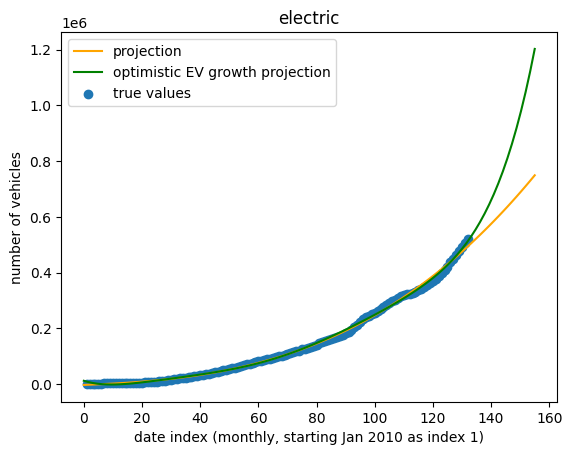
\includegraphics[width=5cm]{imgs/electric_proj.png}
    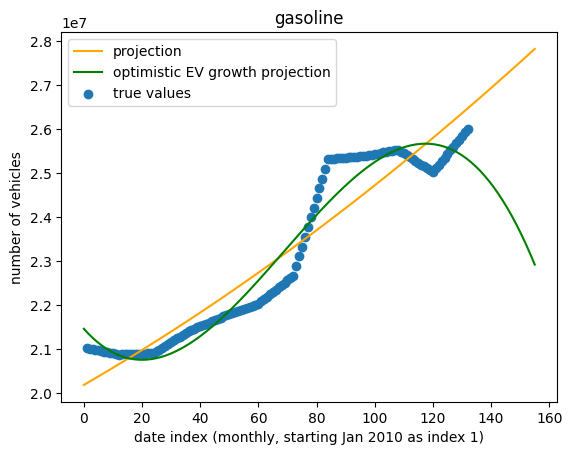
\includegraphics[width=5cm]{imgs/gasoline_proj.png}\\
    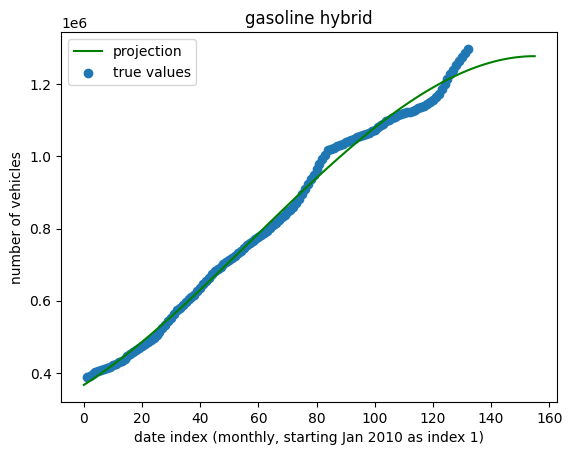
\includegraphics[width=4cm]{imgs/gasoline_hybrid_proj.png}
    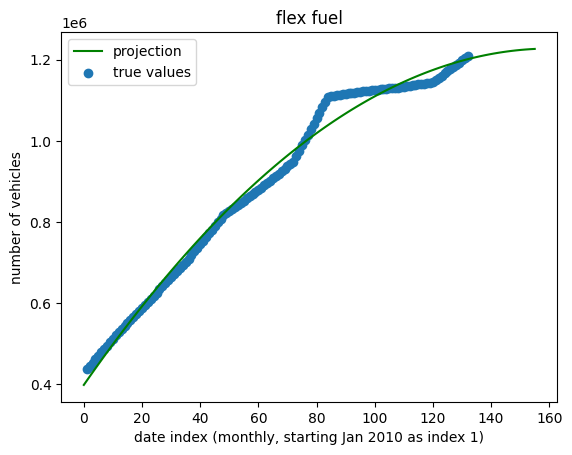
\includegraphics[width=4cm]{imgs/flex_fuel_proj.png}
    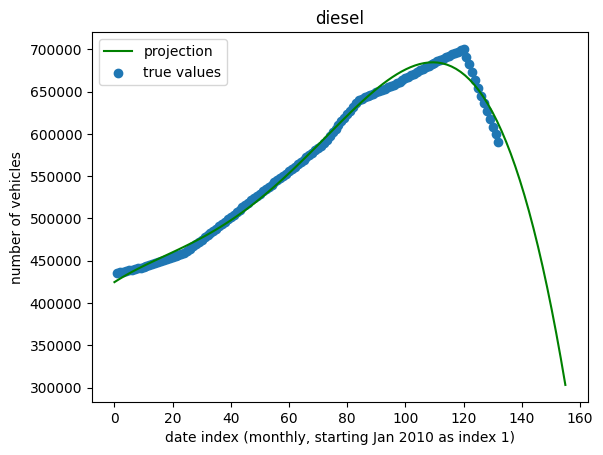
\includegraphics[width=4cm]{imgs/diesel_proj.png}
    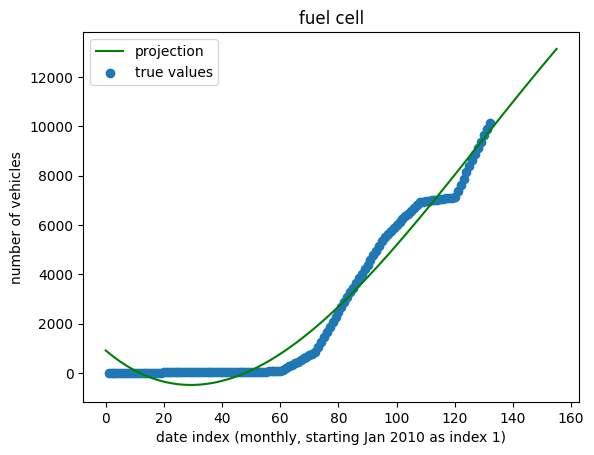
\includegraphics[width=4cm]{imgs/fuel_cell_proj.png}
    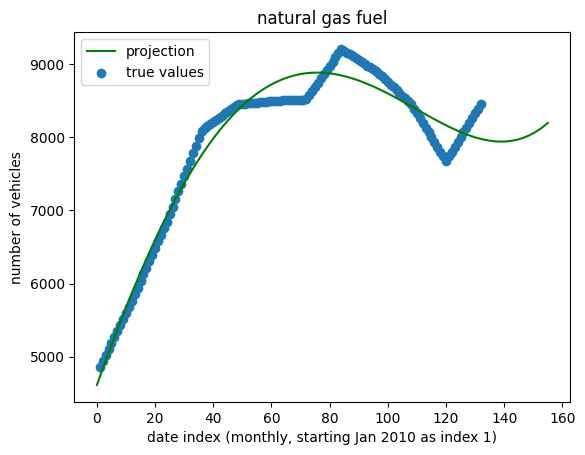
\includegraphics[width=4cm]{imgs/nat_gas_proj.png}
    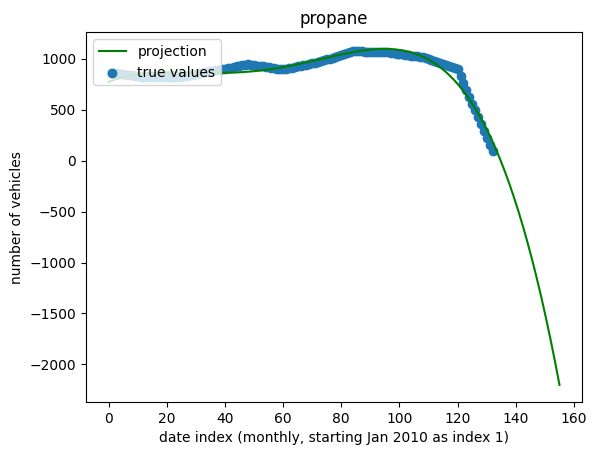
\includegraphics[width=4cm]{imgs/propane_proj.png}
    \caption{\label{registrationprojections} Chosen growth trends for each type of vehicle.}
    \end{center}
\end{figure}


\section{Results}

Assuming that the methods and resources used to  generate energy in California remain relatively the same, we predict monthly emissions from energy generation for August of 2026 for two different vehicle distribution predictions, the first with neutral gasoline and electric vehicle registration growths, the second with an optimistic EV registration growth rate and a slow declining gasoline-vehicle growth rate.

\subsection{Stacked regressor performances}

We use a train-test split of 8-2, with random search over hyperparameters, using R-2 scoring for training and testing scores.

\begin{table}[H]
    \begin{center}
        \begin{tabular}{lll}
        \textbf{Model} & \textbf{Train score} & \textbf{Test score}\\
        RF & 0.93 & 0.83 \\
        Linear regression \& RF & 0.92 & 0.93\\
        Lasso \& RF & 0.95 & 0.95\\
        GB & 0.99 & 0.84 \\
        Linear regression \& GB & 0.98 & 0.98 \\
        Lasso \& GB & 0.98 & 0.96\\
    \end{tabular}
    \end{center}
    \caption{\label{}Accuracy scoring for demand prediction using electric vehicle, plug-in hybrid electric, maximum temperature, and average precipitation data.}
\end{table}
Scoring is roughly comparable for all methods, with slightly increased score for stacking linear regression and GB for demand prediction. We use this method in the below results.

\begin{table}[H]
    \begin{center}
            \begin{tabular}{lll}
        \textbf{Model} & \textbf{Train score} & \textbf{Test score}\\
        RF & 0.83 & 0.64 \\
        Linear regression \& RF & 0.69 & 0.75\\
        Lasso \& RF & 0.79 & 0.79\\
        GB & 0.91 & 0.71 \\
        Linear regression \& GB & 0.82 & 0.81 \\
        Lasso \& GB & 0.93 & 0.89\\
    \end{tabular}
    \end{center}
    \caption{\label{}Accuracy scoring for emissions prediction using vehicle distribution and electricity demand data.}
\end{table}

Stacking lasso and GB performs best among tested models for predicting emissions. We use this method in the below results.

\subsection{\label{results1}Neutral projected vehicle growths}

We generate the following vehicle distribution:

\begin{table}[H]
    \centering
    \begin{tabular}{lcc}
        \textbf{vehicle type} & \textbf{projected number of registrations} & \textbf{\% of all registrations}\\
         electric & 699,835 & 2.22\%\\
         plug-in hybrid electric & 312,033 & 0.99\%\\
         fuel cell & 12,573 & 0.04\%\\
         diesel & 379,989 & 1.21\%\\
         flex fuel & 1,224,642 &  3.89\%\\
         gasoline & 27,575,770 & 87.57\%\\
         gasoline hybrid & 1,276,945 & 4.06\%\\
         natural gas & 8,080 & 0.03\%\\
         propane & 0 & 0\%
    \end{tabular}
    \caption{Projected number of registrations by vehicle type for August 2026}
    \label{table:projection}
\end{table}

This would be an increase of about 51\% (237,584 EVs) from August of 2021.

Using these projections, the average August maximum temperature, of 88$^{\circ}$ F, and average August precipitation of 0.1 inches, we estimate a demand of 27,869,201.23 MWh for the month of August 2026, compared to 27,525,448 MWh from August 2021.

In turn, we project for that month 5,624,180.8  mTCO\(2\) emissions from energy generation, compared to the August 2021 quantity of 5,607,233.68 mTCO\(2\).

\subsection{\label{results2}Optimistic electric vehicle growths}

For the same date, using a more optimistic EV registration growth rate and an eventually declining gasoline-powered vehicle registration rate, we generate the following vehicle distribution:

\begin{table}[H]
    \centering
    \begin{tabular}{lcc}
        \textbf{vehicle type} & \textbf{projected number of registrations} & \textbf{\% of all registrations}\\
         electric & 1,009,995 & 3.64\%\\
         plug-in hybrid electric & 312,033 & 1.12\%\\
         fuel cell & 12,573 & 0.05\%\\
         diesel & 379,989 & 1.37\%\\
         flex fuel & 1,224,642 &  4.41\%\\
         gasoline & 23,517,676 & 84.77\%\\
         gasoline hybrid & 1,276,945 & 4.6\%\\
         natural gas & 8,080 & 0.03\%\\
         propane & 0 & 0\%
    \end{tabular}
    \caption{Projected number of registrations by vehicle type for August 2026 with optimistic EV growth}
    \label{table:projection}
\end{table}

This would be an increase of about 118\% (547,744 EVs) from August of 2021 and a decline of about 8\% for gasoline-fueled vehicles (2,155,196 cars).

Using these projections and the same average August maximum temperature and precipitation values as previously, we estimate a demand of 28,027,557.14 MWh  for the month of August 2026, compared to 27,525,448 MWh from August 2021.

In turn, we project for that month 5,640,539.45 mTCO\(2\) emissions, compared to the August 2021 quantity of 5,607,233.68 mTCO\(2\).


\subsection{\label{comparison}Comparison}

In the case of Section~\ref{results1}, which predicts an increase in EV registrations by 237,584 between August 2021 and August 2026, California would experience 16,947.12 mTCO\(2\) greater emissions that month than in August of 2021.

For Section~\ref{results2}, projections indicate an increase in EV registrations by 547,744 in that timeframe and 16,947.12 mTCO\(2\) more emissions than month than in August of 2021.

In table~\ref{table:emissionscomp}, we compare these values with the estimated emissions from the same number of combustion engine cars in a month, assuming that a typical passenger car emits 4.6 mTCO\(2\) a year, or roughly 0.38 mTCO\(_2\) per month. \citep{caremissions}

Additionally, as we cannot verify emissions projections, we look at another method of estimation. According to one source, \citep{evconsumption} the average EV consumes 406.5 kWh per month, and the \cite{emissionspermwh} calculates an average of 884.2 lbs CO\(_2\) per MWh consumed in the United States---we assume roughly 0.16 mTCO\(_2\) per month per EV. We calculate in the fourth column of table~\ref{table:emissionscomp}, based on these values, the estimated quantity of emissions produced by the number of additional EV registrations.

\begin{table}
    % \centering
    \begin{tabular}{p{4cm}p{4cm}p{2cm}p{2cm}}
        \textbf{EV registration increase} & \textbf{emissions increase} & \textbf{(1)} & \textbf{(2)}\\
         237,584 & 16,947.12 & 98,281.92 & 38,013.44\\
         547,744 & 33,305.77 & 208,142.72 & 87,639.04
    \end{tabular}
    \caption{Projected EV registration increases and monthly emissions increases based on model results, compared to \textbf{(1)} estimated emissions from the same number of gasoline vehicles and \textbf{(2)} estimated emissions generated from EV electricity usage using EPA averages.}
    \label{table:emissionscomp}
\end{table}

In both cases, the emissions due to increased electricity demand represent fractions of those generated by the typical gasoline-powered vehicle. We also notice major discrepancies between this project's estimated emissions and those calculated as the product of the number of EVs and average CO\(_2\) emissions generated per MWh according to the EPA. We may attribute this to two factors: our modeling approach is simply not a good fit and the fact that the EPA average takes into account the entire U.S., where each region releases carbon emissions during energy generation at different rates.

\section{Conclusions}

\subsection{Reflection}

I hoped in my original proposal and approach to develop a more accurate, or at least informed, method of approximating energy consumption as electricity-powered vehicles increase than simply multiplying averages as we did in section~\ref{comparison}. Ultimately, however, this technique may suffice for ballpark approximations of potential emissions and is more understandable.

One main concern regarding the robustness of my approach was the tenuous relation between vehicle distribution numbers and energy demand based on current data, considering the relatively small number of electric and partially electric vehicles in California, which surprised me. I tried to mitigate this with other highly correlated at such as weather, but I fear my understanding of contributors to electricity demand remains shallow and the data too few.

Indeed, the second concern would be data, as I was warned, particularly for vehicle registration, since energy and motor vehicle departments usually only release this data on a yearly basis, which constrains the applicability of machine learning approaches. I extrapolated monthly information, but we would be hard-strapped to find or measure this data on a finer level, such as weekly or daily.

This project could certainly be refined with more specificity for other data like county-level electricity demand and generation and a better understanding of the car market and sales trends. (I do not, for example, have a good sense of what sorts of vehicles use propane and if their number will continue to dwindle or if there exists a purpose for propane-fueled vehicles that precludes their disappearance.) 

Though all thrown together and glossed-over in this single paper, each step in this process merits its own in-depth study: vehicle distribution prediction, electricity demand prediction, and emissions from energy generation.

I believe I got lost in the sauce.

\subsection{Final thoughts}

Though the data and approach used cast a pall of doubt on the real merit of the models applied and certainly on their results, they do seem to reaffirm that emissions engendered by increased energy generation for powering EVs represent a fraction of what would be released directly into the air by an equivalent number of traditional combustion engine vehicles. Not only does this reduce total state emissions in California, but it also reduces air pollution and associated health problems in areas with urban areas with high car densities.

Though the energy generation process will continue to shoulder more of the total carbon emissions for the state, there remains in it great room for improvement, notably through the integration of renewable energies and energy grid connections to more efficiently meet real-time needs with less energy waste, such as through the TransWest Express system, which seeks to bring wind-generated energy from Wyoming to California. \citep{transwest}


\subsection*{Acknowledgment}
To Alp, I recognize the ultimate quality of my work and want to say I still learned a great deal and truly appreciate the thought and energy you put into this class's curriculum and discussions. While it was a disservice to my own learning and growth, I meant no disrespect by not better engaging with you.\\
To both Alp and Dafne, thank you and have a wonderful holiday and new year.

\medskip

\bibliography{refs}

\end{document}